\chapter{Background and Related Work}
% In this chapter, we detail the background and prior research that underpins the work described in later chapters. Further, we include an explanation of the theoretical concepts, both reinforcement learning and graph neural networks, which we have used extensively in this work.

\section{Introduction to Deep Learning Models}
This section discusses the way in which machine learning models are represented for efficient execution on physical hardware devices. First, we discuss how the mapping of tensor operations to computation graphs is performed followed by an overview of recent approaches that optimise computation graphs to minimise execution time.

Over the past decade, there has been a rapid development of various deep learning architectures that aim to solve a specific task. Common examples include convolutional networks (popularised by AlexNet then ResNets, etc), transformer networks that have seen use in the modelling and generation of language. Recurrent networks that have shown to excel at learning long and short trends in data.

Importantly, the fundamental building blocks of the networks have largely remained unchanged.  As the networks become more complex, it becomes untenable to manually optimise the networks to reduce the execution time on hardware. Therefore, there is extensive work in ways to both automatically optimise the models, or, alternatively apply a set of hand-crafted optimisations.

Computation graphs are a way to graphically represent both the individual tensor operations in a model, and the connections (or data-flow) along the edges between nodes in the graph. Figure \ref{fig:bg:perceptron} shows how the expression, $y = \texttt{ReLU}(\mathbf{w} \cdot \mathbf{x} + b)$, can be represented graphically in a computation graph.

\begin{figure}[ht]
  \centering
  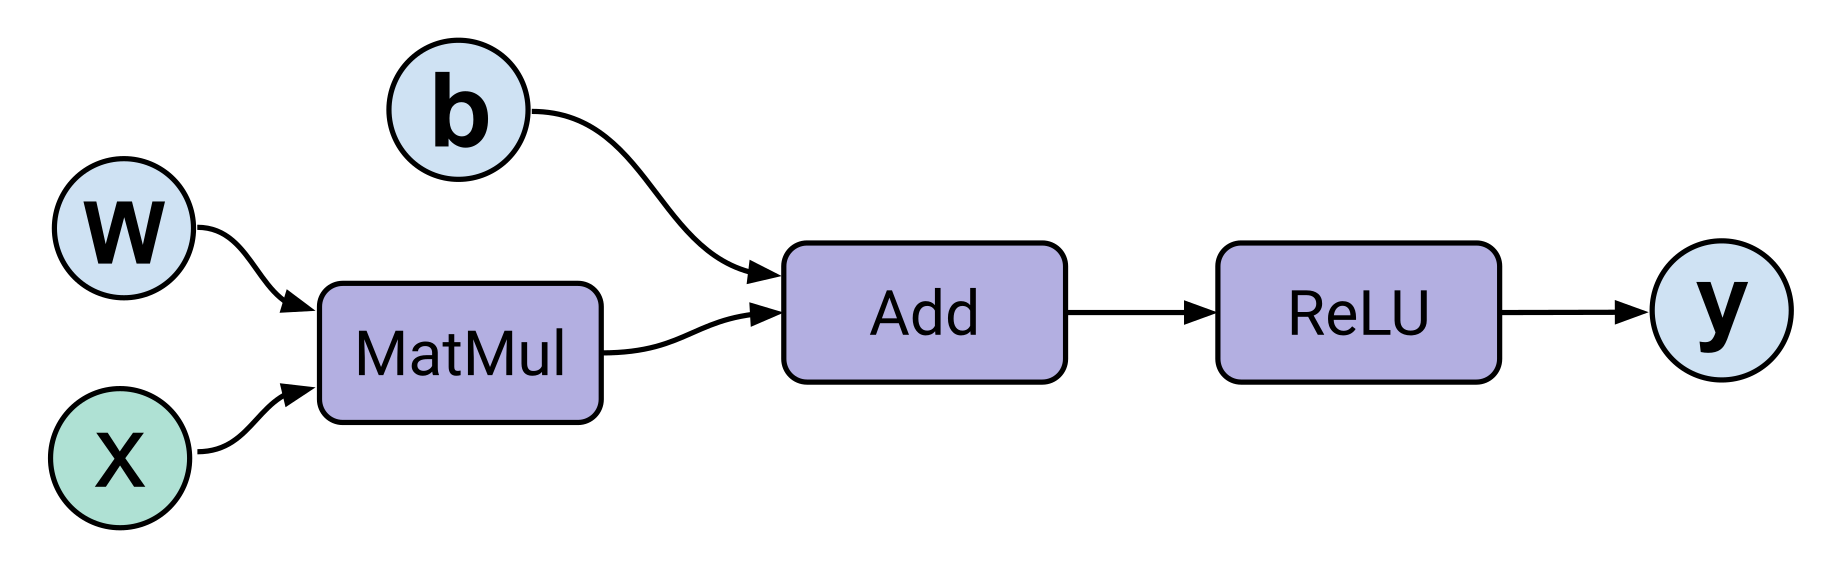
\includegraphics[width=0.75\columnwidth]{sections/2background/images/dataflow}
  \caption[Single perceptron as a dataflow (computation) graph]{The operations shown in purple are the nodes of the computation graph which take an arbitraty number of inputs, performs a computation at the node and produces an output. The blue nodes represent the input nodes for tensors. The directed edges show the flow of tensors through the graph.}
  \label{fig:bg:perceptron}
\end{figure}

Similarly, the whole model can be converted into a stateful dataflow graph in this manner. By using a stateful dataflow (or computation) graph, we can use any optimisation technique for backpropagation of the model loss though the graph [TODO rewrite last sentence]. We consider two key benefits of this representation. First, we can execute the model on any hardware device as the models have a single, uniform representation. Secondly, it allows for pre-execution optimisations based on the host device, for example, we may perform different optimisations for executing on a GPU compared to a TPU.

\subsection{Current approaches to optimising deep learning models}

Due to the prevalence and importance of machine learning, especially deep networks, there is a focus on finding ways decrease the inference runtime and by extension, increasing the model throughput. All major frameworks such as TensorFlow \cite{Tensorflow2015-whitepaper}, PyTorch \cite{pytorch}, MXNet \cite{chen2015mxnet}, and Caffe \cite{jia2014caffe} have some level of support for performing pre-execution optimisations. However, the process of performing such optimisations is often time-consuming and cannot be completed in real-time. Rather, it is common to use a deep learning optimisation library such as cuDNN \cite{chetlur2014cudnn} or cuBLAS \cite{cublas2008} that instead directly optimise individual tensor operations.

%common machine learning framework is designed to greedily apply a set of pre-defined substitutions to an input graph in an attempt to optimise the graph. TensorFlow made use of low-level libraries such as cuBLAS \cite{cublas2008} for optimised matrix operations and cuDNN \cite{chetlur2014cudnn} for convolutional kernels. Furthermore, TensorFlow also contains a set of 155 substitutions that are implemented in 53,000 lines of code; to complicate matters, new operators are continuously proposed, such as grouped or transposed convolutions, all of which leads to a large amount of engineering effort required to maintain the library.

%TensorRT \cite{tensorrt2017} provides a high-performance SDK to optimise the inference of models via a combination of techniques such as layout and tensor fusion, auto-tuning kernels, and multi-stream execution. The SDK acts as both the optimisation and execution engine that lies between the ML framework and physical hardware. Importantly, it is not involved during the training process, rather, it assumes for the best possible performance that the developer 

Alternatively, TVM and TensorRT can be used to optimise deep learning models and offer greater performance gains compared to the more commonly used frameworks such as TensorFlow and PyTorch. They also use greedy rule-based optimisation approaches. TODO - either expand or remove

Rather than using a rule-based optimisation approach, it is possible to use more sophisticated algorithms to optimise deep learning models at the expense of computation time. Jia et al. used a cost-based backtracking search to iteratively search through the state space of possible graphs that are provably equivalent \cite{jia2019taso}. As opposed to using rule-based optimisation that applied hand-crafted optimisations, TASO generates the candidate subgraphs automatically and formally proves the transformations are equivalent using an automated theorem prover. Furthermore, Jia et al. showed that by jointly optimising both the data layout of the subgraph transformation, and the transformation itself, TASO achieves a speedup compared to performing the operations sequentially.

A key benefit of using a cost-based approach is that the search can take into account far more complex interactions between the transformed kernels. For example, if we apply a series of transformations $T_1, \cdots, T_i$, the runtime may increase, and, due to the first set of transformations, we can now apply $T_{i + 1}, \cdots, T_{i + j}$, after all transformations have been applied, it is possible that we see a net decrease in runtime. By increasing the search space of transformations in this way, Jia et al. showed that it is possible to increase the runtime of deep learning models by up to 3x \cite{jia2019taso, jia2019optimizing} compared to baseline measurements.


\section{Reinforcement Learning}
Reinforcement learning (RL) is a sub-field in machine learning, broadly, it aims to compute a control policy such that an agent can maximise its cumulative reward from the environment. It has powerful applications in environments where a model that describes the semantics of the system are not available and the agent must itself discover the optimal strategy via a reward signal.

- TODO Should also mention POMDPs?

Formally, RL is a class of learning problem that can be framed as a Markov decision processes (MDP) when the MDP that describes the system is not known \cite{bellman1957}; they are represented as a 5-tuple $\langle \mathcal{S}, \mathcal{A}, \mathcal{P}_a, \mathcal{R}_a, \rho_0 \rangle$ where:

\begin{itemize}
  \item $\mathcal{S}$, is a finite set of valid states
  \item $\mathcal{A}$, is a finite set of valid actions
  \item $\mathcal{P}_a$, is the transition probability function that an action $a$ in state $s_t$ leads to a state $s'_{t+1}$
  \item $\mathcal{R}_a$, is the reward function, it returns the reward from the environment after taking an action $a$ between state $s_t$ and $s'_{t+1}$
  \item $\rho_0$, is the starting state distribution
\end{itemize}

% TODO: add citations
We aim to compute a policy, denoted by $\pi$, that when given a state $s \in \mathcal{S}$, returns an action $a \in \mathcal{A}$ with the optimisation objective being to find a control policy $\pi^*$ that maximises the \textit{expected reward} from the environment defined by \ref{equ:expec-rew}. Importantly, we can control the `far-sightedness' of the policy by tuning the discount factor $\gamma \in [0, 1)$. As $\gamma$ tends to 1, the policy will consider the rewards further in the future but with a lower weight as the distant expected reward may be an imperfect prediction.

\begin{equation}
  \label{equ:expec-rew}
  \pi^* = \argmax_\pi~\mathbb{E} \left[ \sum^\infty_{t=0} \gamma^t~\mathcal{R}_t \right]
\end{equation}

Classic RL problems are formulated as MDPs in which we have a finite state space, however, such methods quickly become inefficient with large state spaces that we consider with applications such as Atari and Go. Therefore, we take advantage of modern deep learning function approximators, such as neural networks, that makes learning the solutions far more efficient in practise. We have seen many successfully applications in a wide range of fields, for example, robotic control tasks \cite{openai2019solving}, datacenter power management, device placement, and, playing both perfect and imperfect information games to a super-human level. Reinforcement learning excels when applied to environments in which actions may have long-term, inter-connected dependencies that are difficult to learn or model with traditional machine learning techniques.

In the following sections we discuss the two key paradigms that exist in reinforcement learning and the current research in both areas and the application to systems tasks.

\subsection{Model-Free and Model-Based RL}

Model-free and model-based are the two main approaches to reinforcement learning, however, with recent work such as \cite{app10196685, kaiser2020modelbased, robine2021smaller}, the distinction between the two is becoming somewhat nebulous; it is possible to use a hybrid approach that aims to improve the sample efficiency of the agent by training model-free agents directly in the imagined environment.

The major branching point that distinguishes between model-free and model-based approaches is in what the agent learns during training. A model-free agent, in general, could learn a governing policy, action-value function, or, environment model. On the other hand, model-based agents commonly either learn an explicit representation of the parameterised policy $\pi_\theta$ using planning, such as AlphaZero \cite{silver2017mastering} or ExIt \cite{anthony2017thinking}. Alternatively, we can use use data augmentation methods to learn a representation of the underlying environment behaviour, and either only use fictitious model, or augment real experiences to train an agent in the domain \cite{kaiser2020modelbased, feinberg2018modelbased, freeman2019learning}.

Understandably, a relevant question is why one would prefer a model-free over model-based approach and what are the benefits of the respective methods. The primary benefit of model-based RL is that is has far greater sample efficiency, meaning, the agent requires in total, less interactions with the real environment than the model-free counterparts. If we can either provide, or learn, a model of the environment it allows the agent to plan ahead, choosing from a range of possible trajectories its actions to maximise its reward. The agent that acts in this ``\textit{imagined}'' or ``\textit{hallucinogenic}'' environment can be a simple MLP \cite{ha2018worldmodels} to a model-free agent trained using modern algorithms such as PPO, A2C or Q-learning. Further, training an agent in the world model is comparatively cheap, especially in the case of complex systems environments where a single episode an be on the order of hundreds of milliseconds.

Unfortunately, learning a model of the environment is not trivial. The most challenging problem that must be overcome is that if the model is imperfect, the agent may learn to exploit the models deficiencies, thus making it effectively useless in the real environment.

Model-based approaches have been successfully applied in various domains such as board games, video games, systems optimisation and robotics. Despite the apparent advantages of model-based RL with regards to reduced computation time, model-free reinforcement learning is by far the most popular approach and massive amounts of compute, typically by distributed training on clusters of GPUs/TPUs, is required overcome the sample inefficiency of model-free algorithms.

\subsection{World Models}
World models, first introduced by Ha and Schmidhuber, motivated and described an approach to model-based reinforcement learning in which we learn a model of the real environment using function approximators and train an agent using only predictions from the world model. Figure \ref{fig:bg:mb-rl} shows the design to utilise a world model as substitute for the real environment. In practise, a world model can be broken down into three main components. A visual model, $V$, that encodes the input into a latent vector $z$, a memory model, $M$ the integrates the historical state to produce a representation that can be used as planning for future actions and rewards. Finally, a controller, $C$ that uses both $V$ and $M$ to predict an action from the action set, $a \in \mathcal{A}$.

\begin{figure}[ht]
  \centering
  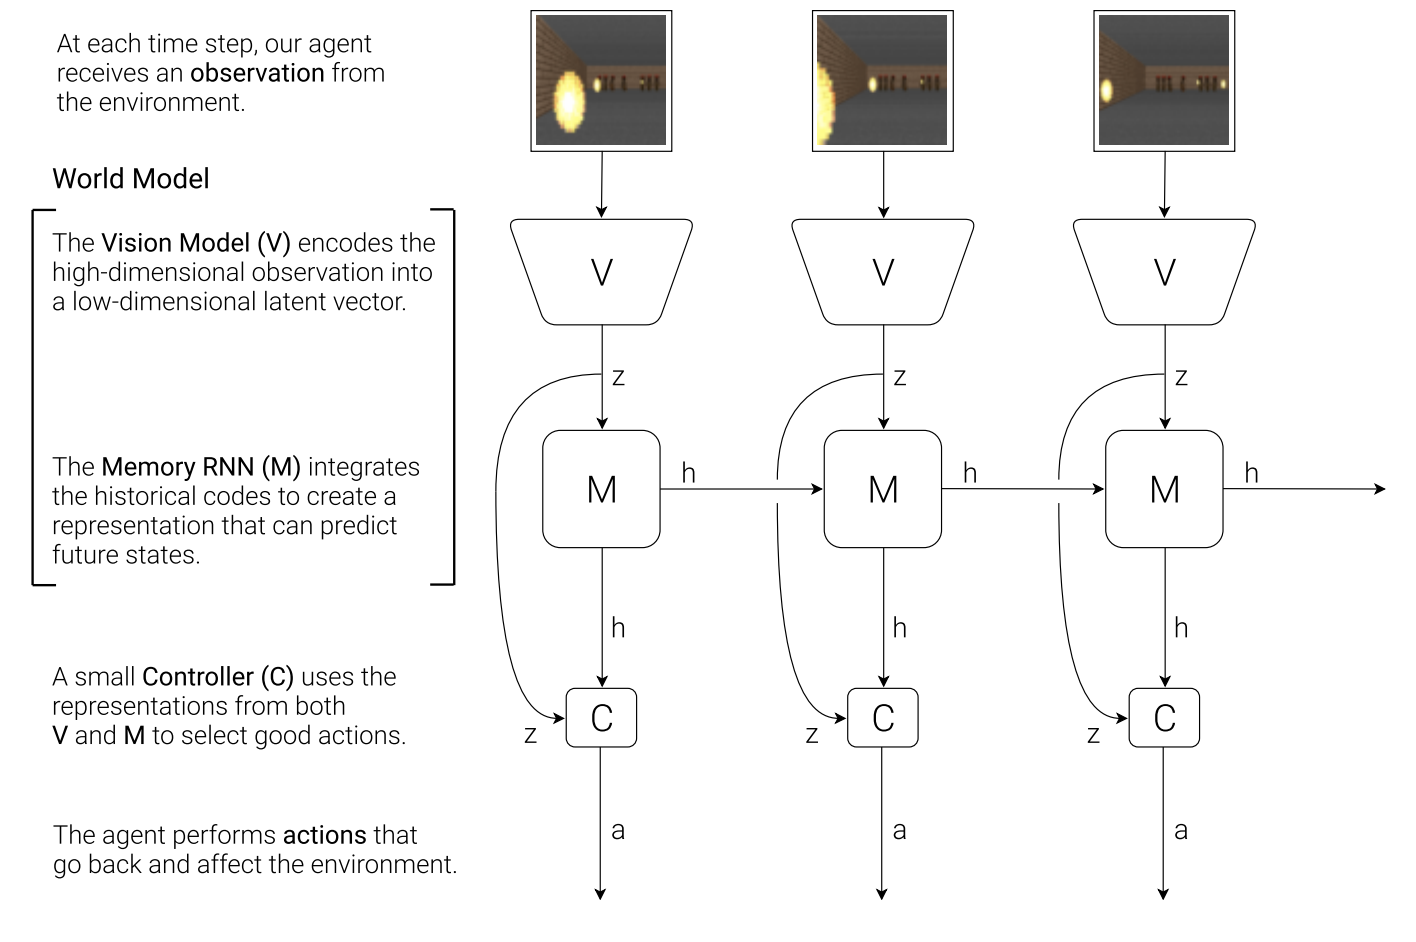
\includegraphics[width=0.75\columnwidth]{sections/2background/images/mb-rl.png}
  \caption[Model-based Reinforcement Learning End-To-End System]{Diagrammatic representation of a world-model made up from an encoder (V) that transforms the input into latent space, a `memory' module, M, that learns the behaviour of the environment from the latent vector $z$ and a controller, C, that is trained using the latent vector of the encoder and the output features from the memory to choose an action which is either applied to the real or imagined environment. Figure adapted from \cite{ha2018worldmodels}.}
  \label{fig:bg:mb-rl}
\end{figure}

Typically, a world model is trained using rollouts of the real environment that have been sampled using a random agent acting in the environment. The aim is to learn to accurately predict, given a state $s_t$, the next state $s_{t+1}$ and the associated reward $r_{t+1}$. After training, the controller, $C$, can either learn using only observations from the world model, so called ``training in a dream''. Alternatively, the world model can be used to augment the observations from the real environment samples or used only for planning. To construct the world model, if the environment is simple and deterministic, it is possible to use a deep neural network to act as the world model, however, for environments that are only partially observable, a more complex model is required such as Recurrent Neural Networks (RNNs) or Long-short term memory (LSTMs). The following two sub-sections describe the fundamental concepts required to construct a world model.

\subsubsection{Mixture Density Networks}
Mixture Density Networks (MDNs) are a class of neural networks first described by Christopher Bishop \cite{bishop1994mixture} that were designed to deal with problems where there is an inherent uncertainty in the predictions. Given an input to the network, we wish to output a range of possible outputs conditioned on the input where we can assess the probability of each outcome. MDNs are commonly parameterised by a neural network that is trained using supervised learning and outputs the parameters for multiple mixture of Gaussians.

\subsubsection{Recurrent Neural Networks}
Recurrent Neural Networks are class of neural networks that allows for previous outputs to be re-used as inputs to sequential nodes while maintaining and updating their own hidden state. Primarily, RNNs are commonly used in the field of speech recognition and natural language processing as they can process inputs of an arbitrary length with a constant model size. In practise however, RNNs suffer from being unable to utilise long chains of information due to the vanishing/exploding gradient problem; the gradient can change exponentially changing in proportion to the number of layers in the network \cite{Hochreiter:01book}.

Motivated by the desire to overcome the limitations of RNNs, Hochreiter et al. \cite{hochreiter1997long} developed long-short term memory by describing Constant Error Carousel (CECs). The idea was further improved by Gers et al. \cite{gers1999learning} with the modern LSTM that is made up of four gates, each with a specific purpose that influences the behaviour of each cell and in combination, the properties of the network as a whole. Figure \ref{fig:bg:lstm} shows the internal structure of an LSTM module.

\begin{figure}[ht]
  \centering
  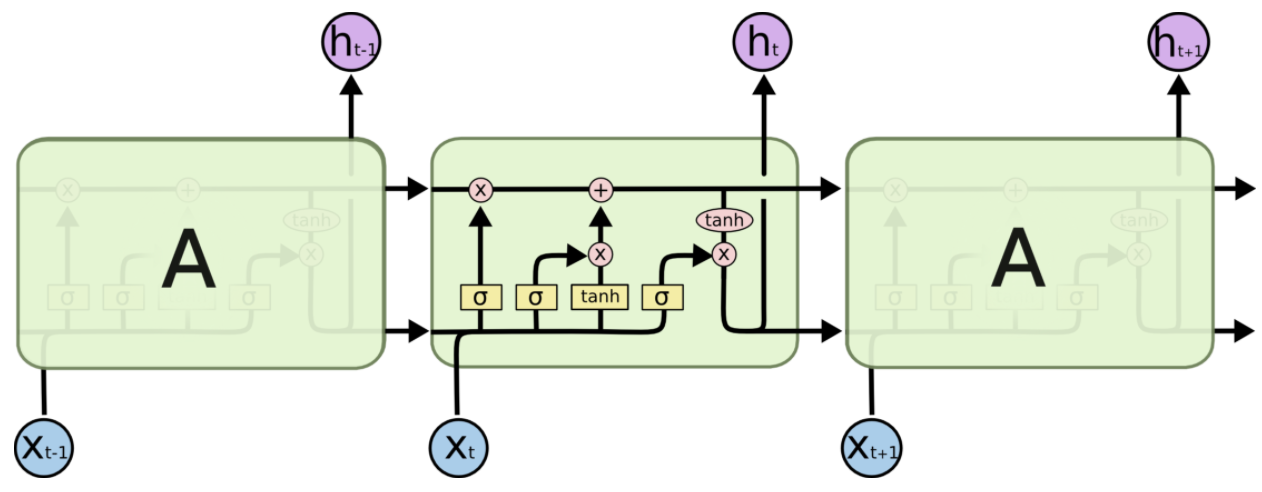
\includegraphics[width=0.75\columnwidth]{sections/2background/images/lstm.png}
  \caption[Structure of an unrolled LSTM]{LSTM}
  \label{fig:bg:lstm}
\end{figure}

An LSTM can be described used four ``gates'', where a gate influences a property of the behaviour of the LSTM cell. The \textit{forget} gate dictates if the information stored in the cell should be erased by observing the inputs $[h_{t-1}, x_t]$ it outputs a value in the range $[0, 1]$, using the sigmoid function $\sigma$, where $1$ means to completely forget the state. Secondly, the \textit{input} gate calculates the new information to be stored in the cell state, generating a vector of candidates $\tilde{C}_t$. The \textit{update} gate is to determine how much of the past state sequence should be considered using the outputs from the \textit{forget} gate, the prior state $C_{t-1}$ and the input gate $\tilde{C}_t$. Finally, the \textit{output} gate determines the LSTM cell output based on the current, filtered state of the cell.

\begin{center}
  \begin{align*}
    f_t &= \sigma (W_f \cdot [h_{t-1}, x_t] + b_f) && (1)~\text{Forget gate} \\
    i_t &= \sigma (W_i \cdot [h_{t-1}, x_t] + b_i) && (2)~\text{Input gate} \\
    \tilde{C}_t &= \tanh (W_C) \cdot [h_{t-1}, x_t] + b_C) && (3)~\text{Candidate value} \\
    C_t &= f_t C_{t-1} + i_t \tilde{C}_t && (4)~\text{Update previous cell state} \\
    o_t &= \sigma (W_o [h_{t-1}, x_t] + b_o) && (5)~\text{Output gate} \\
    h_t &= o_t \cdot \tanh (C_t) && (6)~\text{Hidden state}
  \end{align*}
\end{center}

There are a number of popular varients of LSTM cells such as peephole LSTMs, GRUs, Grid LSTMs and ConvLSTM. There are many areas which have been revolutionised by the usage of LSTM cells in the network architecture. As we will describe in [TODO: ref chapter], LSTM cells are a key to allow world models to learn to simulate the behaviour of the environment state-action transitions.

\section{Graph Neural Networks}

Graph neural network are a class of neural network that has seen considerable focus in recent years, with many successful applications being devised around the central idea of leveraging the structure of the graph input to aid in predicting attributes about the graph itself. The motivation factor for the use of graph networks is that, similar to the way in which convolutional neural networks revolutionised the application of neural networks to high dimensional inputs with images, video and audio - we desire an efficient way to generalise CNNs onto graphs.

Battaglia et al. \cite{battaglia2018relational} defines a generalisable framework for entity/relation based reasoning with three main operators that act on edges, nodes, and on global features using user-defined functions. Within the framework described by Battaglia et al., a graph is defined as $G = (u, V, E)$ where $u$ are the global attributes, $V = {\mathbf{v}_i}_i={1:N^v}$ is the set of vertices (with a cardinality of $N^v$) and finally, $E = {(\mathbf{e}_k, r_k, s_k)}_k={1:N^e}$ is the set of edge attributes with their sources and corresponding vertices.

{\SetAlgoNoLine
\begin{algorithm}[H]
 \setstretch{1.0}
 \For{$k \in \lbrace1\dots N^e \rbrace$}{
   $\mathbf{e}'_k \leftarrow \phi^e (\mathbf{e}_k, \mathbf{v}_{r_k}, \mathbf{v}_{s_k}, \mathbf{u})$
 }

 \For{$i \in \lbrace1\dots N^n \rbrace$}{
   \textbf{let} $E'_i = \lbrace (\mathbf{e}'_k, r_k, s_k) \rbrace_{r_k=i, k=1:N^e}$ \\
   $\bar{\mathbf{e}}'_i \leftarrow \rho^{e\rightarrow v} (E'_i)$ \\
   $\bar{\mathbf{v}}'_i \leftarrow \phi^{v} (\bar{\mathbf{e}}'_i, \mathbf{v}_i, \mathbf{u})$
 }

 \textbf{let} $V' = {\mathbf{v'}_{i=1:N^v}}$\\
 \textbf{let} $E' = {(\mathbf{e}'_k, r_k, s_k)}_{k=1:n^e}$\\

 $\bar{\mathbf{e}}' \leftarrow \rho^{e\rightarrow u} (E')$ \\

 $\bar{\mathbf{v}}' \leftarrow \rho^{v\rightarrow u} (V')$ \\

 $\bar{\mathbf{u}}' \leftarrow \phi^{u} (\bar{\mathbf{e}}', \bar{\mathbf{v}}', \mathbf{u})$ \\

 \Return{$(E', V', \mathbf{u}')$}

 \caption{Computation in a full GN block. Adapted from \cite{battaglia2018relational}}
 \label{algo2}
\end{algorithm}}

We can define three update functions and three \textit{aggregation} function. The update functions are $\phi^e$, $\phi^v$ and $\phi^u$ for edges, vertices and globals respectively. The aggregation functions are $\rho^{e \rightarrow v} (E'_i)$, $\rho^{e \rightarrow u} (E')$, and $\rho^{v \rightarrow u} (V')$, for edges, vertices and globals respectively. To perform a single update given a set of input edges and vertices, we simply apply the three update and aggregation functions sequentially in the order of edges $\rightarrow$ vertices $\rightarrow$ globals. Algorithm \ref{algo2} describes, in general, the algorithm to perform an update of a graph block.

- Graph Auto-encoders

% An inductive bias is a set of assumptions that allows for the algorithm to prioritise one solution over another, while being independent from the previously observed data. 

